\chapter{Upcoming plan}

\section{The camera module}

After having discussed mainly the solutions and implementations of the soft modules in the system, we must move on to the main one that is considered to be the eyes of the thesis, which is the camera module. This Section will discuss what parts are in a camera module and represent some images of a real one we built.

We can easily find the camera modules' parts from any retailer selling electrical components, robots, and Arduino kits. Additionally, in the current era of e-commerce, it is easier for us to find and compare those components that we need online. The parts required to build a camera module are listed below.

First, we need a camera part, and ESP32-CAM is the perfect one for this role. It is inexpensive and easy to use, making it ideal for our thesis that requires complex functions like image tracking and recognition. Furthermore, it integrates Wi-Fi, traditional Bluetooth, which help us in sending the images to the user's smartphone for the next steps in translating sign language.

Secondly, we need a converter adapter to help us sideload the program into the camera module. Besides, the third part that we need is the ultrasonic sensor mentioned in the Section \ref{sec:locationDetection}. It plays a role in location detection, which will tell the system the distance between hands and the camera module. Last but not least, this camera module needs a battery to power the whole module, and we reckon that the volume of about 100 mAh is fine.

Furthermore, there must be a box to store all the above parts. With the help of current 3D printing technology, we design that package on Tinkercad, an online 3D modeling program that runs on the web browser. After getting all the necessary components, we tried to put them all together and get the result below.

\begin{figure}[H]
	\centering
	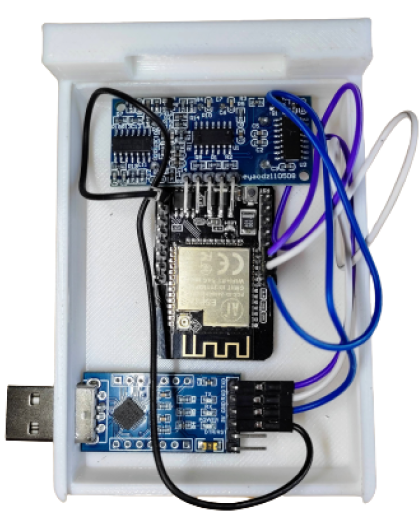
\includegraphics[width=0.45\textwidth]{img/Chap5/Prototype_View_inside.png}
	\caption{The components inside the camera module prototype}
\end{figure}

\begin{figure}[H]
	\centering
	\begin{subfigure}[b]{0.45\textwidth}
		\centering
		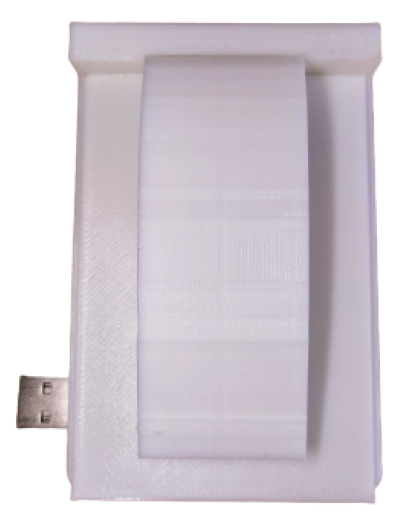
\includegraphics[width=\textwidth]{img/Chap5/Prototype_View_above.png}
	\end{subfigure}
	\hfill
	\begin{subfigure}[b]{0.46\textwidth}
		\centering
		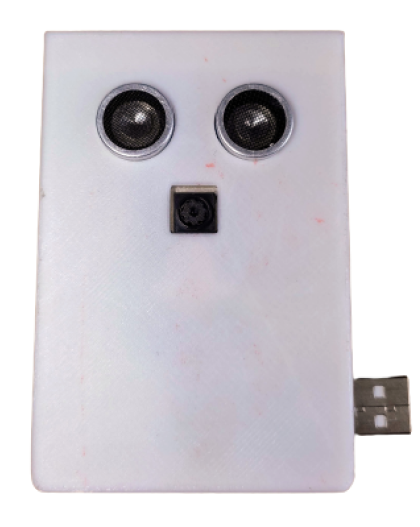
\includegraphics[width=\textwidth]{img/Chap5/Prototype_View_under.png}
	\end{subfigure}
	\caption{Views of the camera module prototype from the above and under}
\end{figure}

\begin{figure}[H]
	\centering
	\begin{subfigure}[b]{0.45\textwidth}
		\centering
		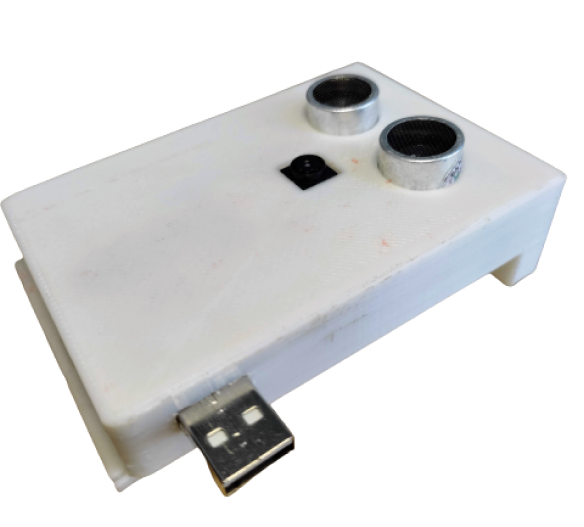
\includegraphics[width=\textwidth]{img/Chap5/Prototype_View_side_1.png}
	\end{subfigure}
	\hfill
	\begin{subfigure}[b]{0.45\textwidth}
		\centering
		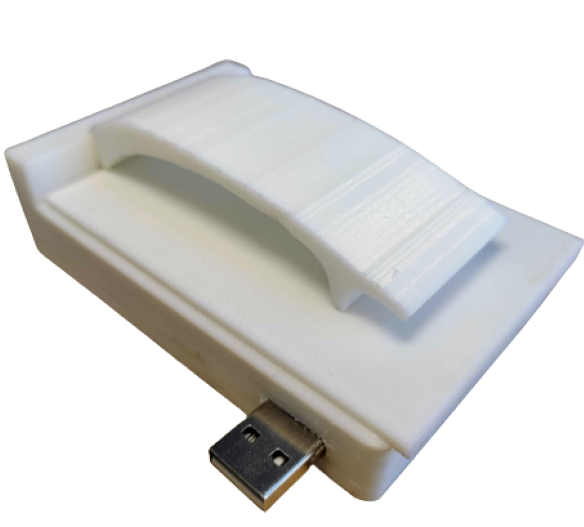
\includegraphics[width=\textwidth]{img/Chap5/Prototype_View_side_2.png}
	\end{subfigure}
	\caption{Views of the camera module prototype from the sides}
\end{figure}

Nevertheless, due to the smallest number that a 3D printer can print, the box's cover is a bit hard to put in. And the hanger that helped hang the box on the hat is not as flexible as we thought, so it needs a redesign.

\section{App design}

The application must satisfy user experience, and user interface demands. And during the research phase of the thesis, we did design a prototype for the application, including two more features besides the main one. Those features are a sign language dictionary and a learning system. We will talk more about those features in the later sections.

Before going through the design of this application, we must state that they do not cover all the screens needed for the application yet. And they are not the final design that we have. However, we have some conventions when designing this prototype, such as the corner is rounded and the colors are pale, not too bright, to make the users feel calm somehow and comfortable when using the application.

\begin{figure}[H]
	\centering
	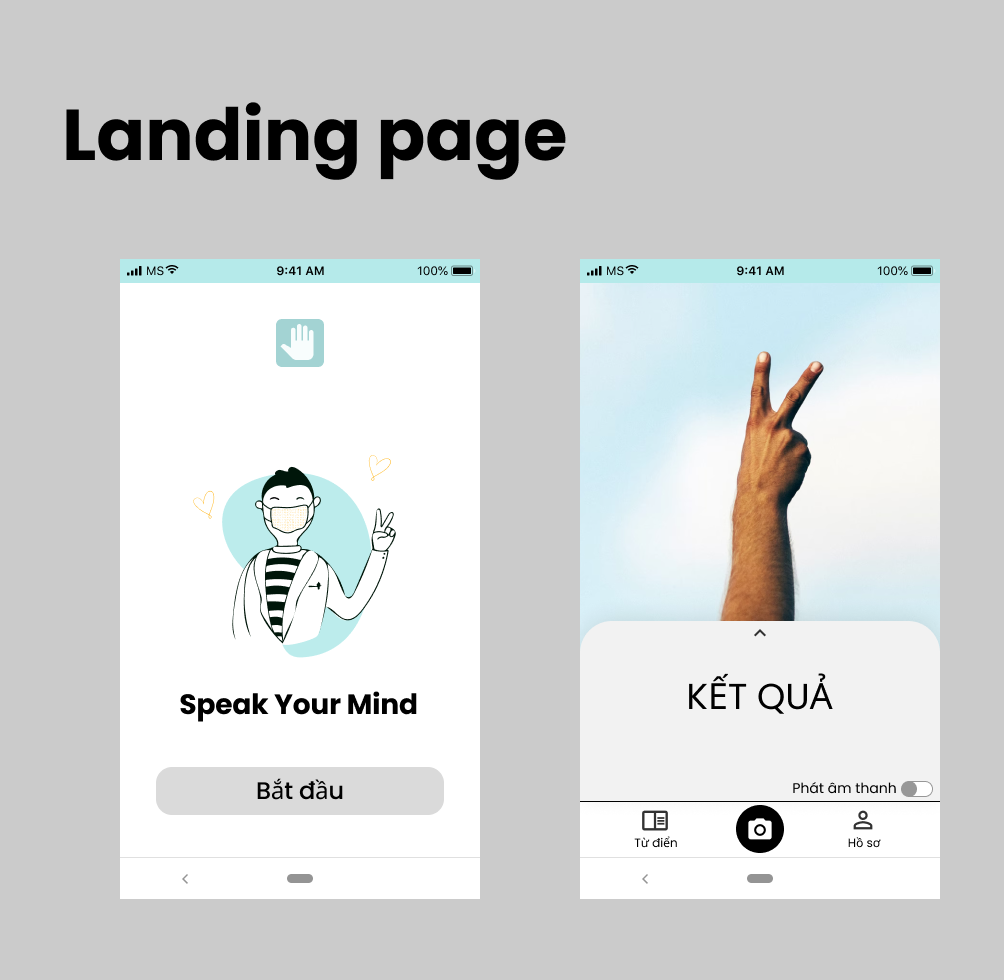
\includegraphics[width=0.8\textwidth]{img/Chap5/Landing_page.png}
	\caption{The landing page of the application}
\end{figure}

\begin{figure}[H]
	\centering
	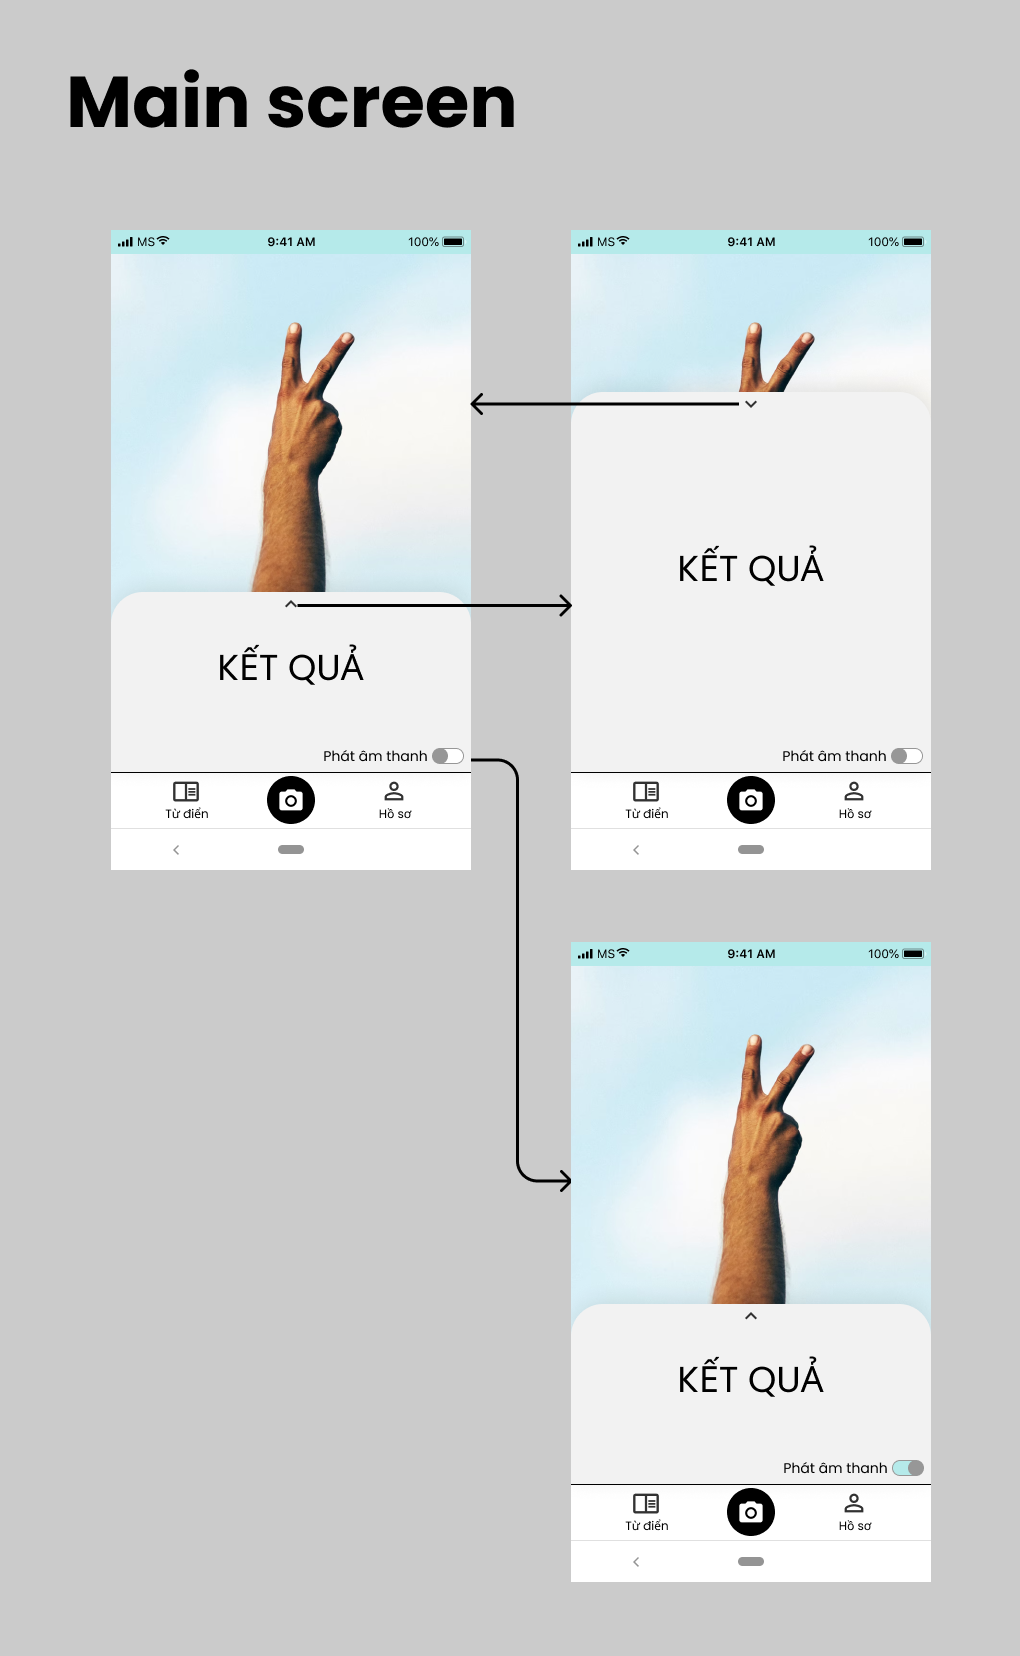
\includegraphics[height=0.8\textheight]{img/Chap5/Main_screen.png}
	\caption{The main screen of the application}
\end{figure}

\begin{figure}[H]
	\centering
	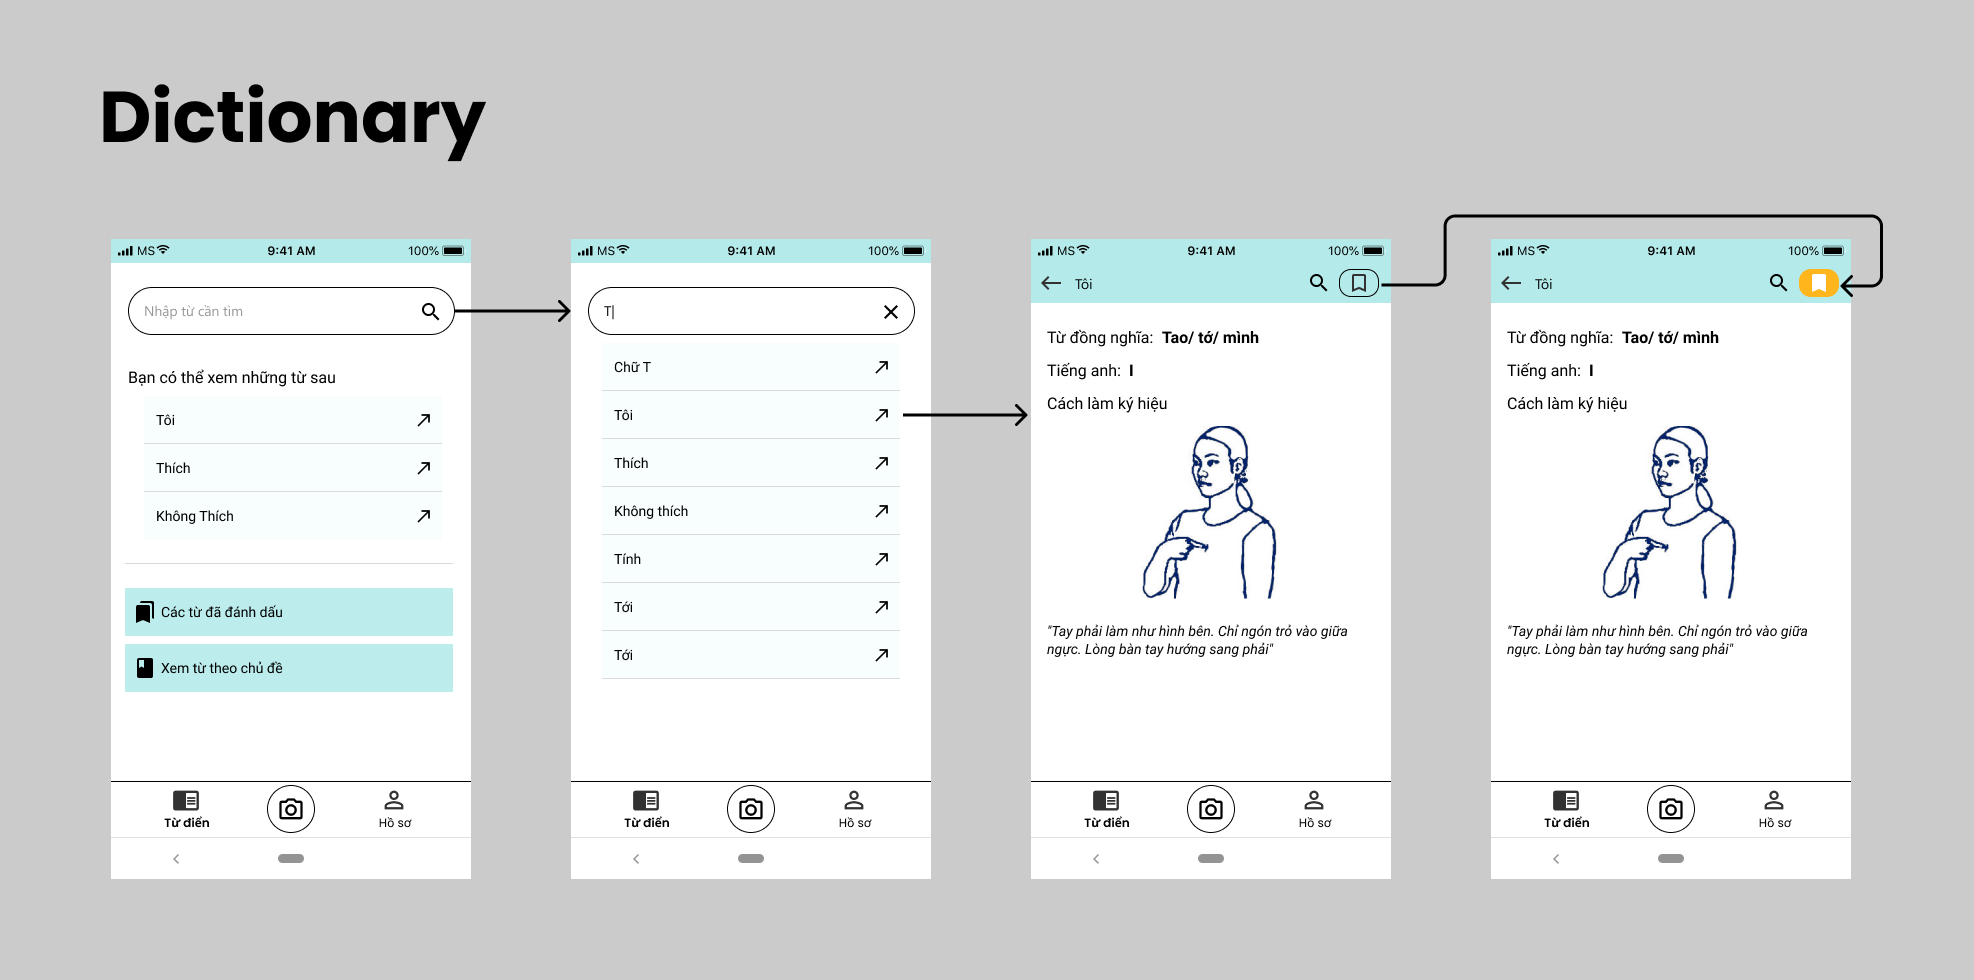
\includegraphics[width=\textwidth]{img/Chap5/Dictionary.png}
	\caption{The main screen of the application}
\end{figure}

\begin{figure}[H]
	\centering
	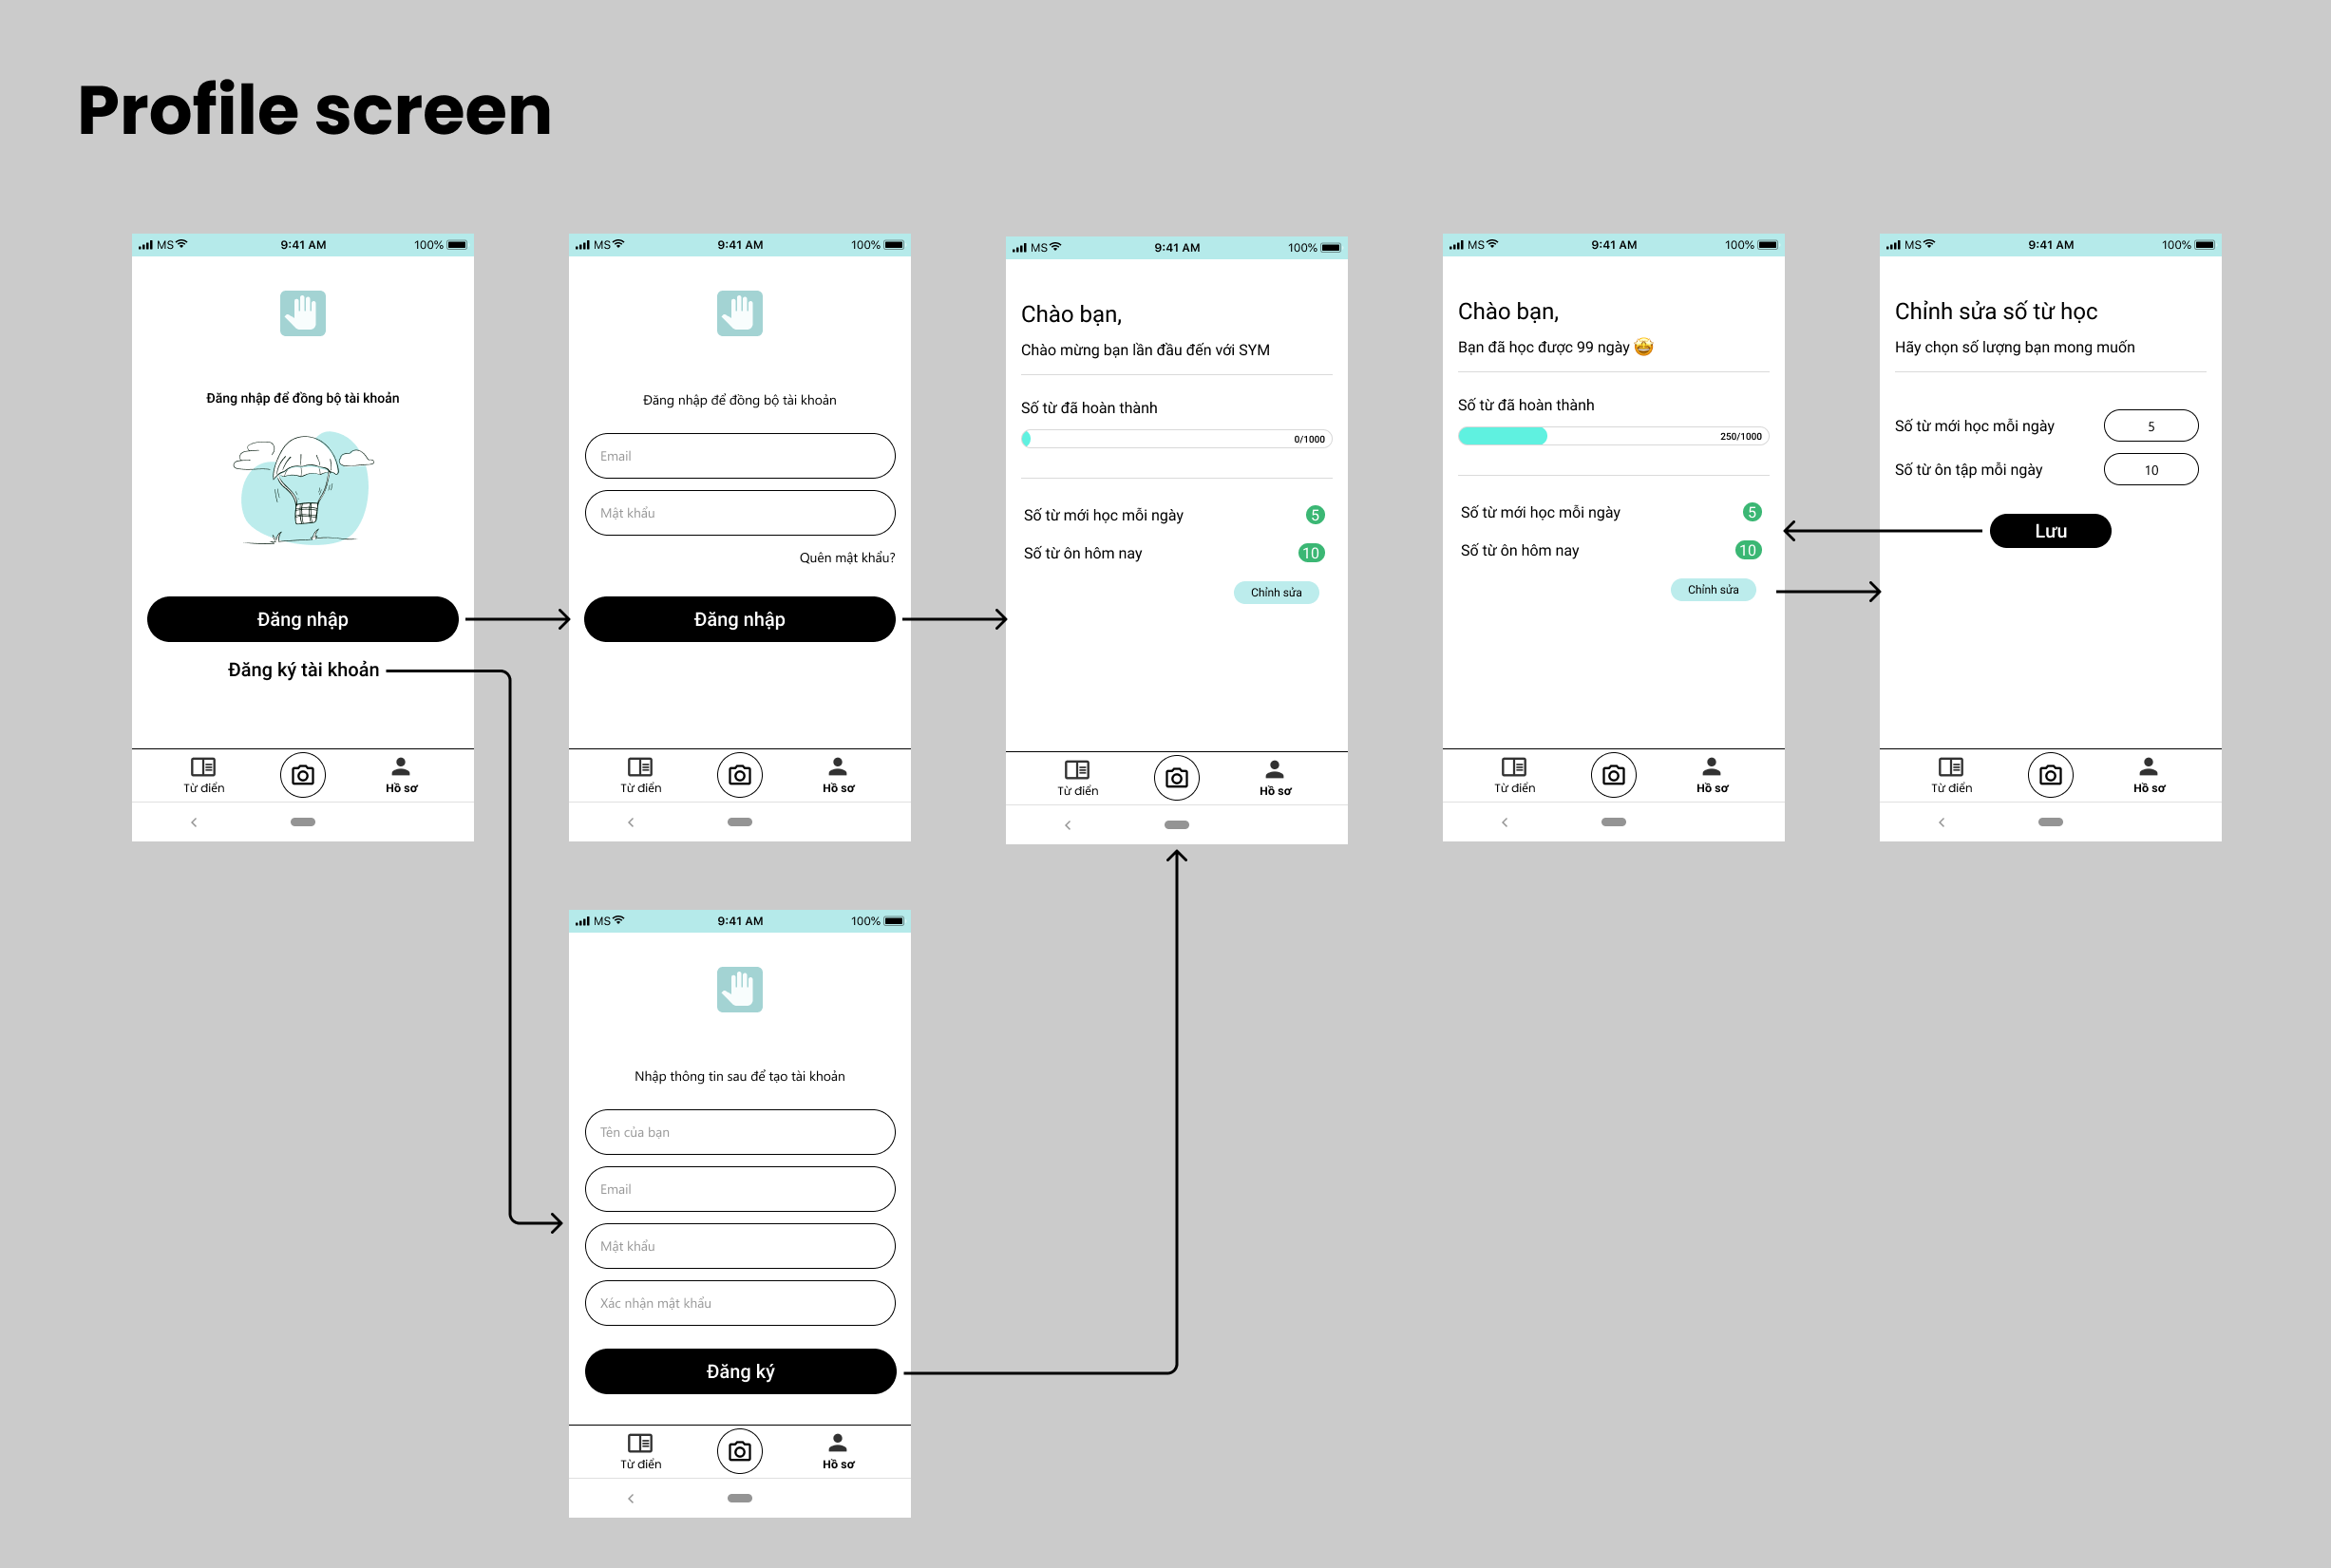
\includegraphics[width=\textwidth]{img/Chap5/Profile_screen.png}
	\caption{The main screen of the application}
\end{figure}

\section{New features and plan for thesis}

To expand the group of people using this application, we will implement additional features into the main application to help ordinary people learn and know more about sign language. Those features are a sign language dictionary and a learning system that help people learn sign language more efficiently.

\begin{itemize}
	\item \textbf{Sign language dictionary:} like any other dictionary, but dictionary has another element, which is containing the videos to illustrate the sign of the words.
	\item \textbf{Learning system:} apply the spaced repetition technique, which help people learn much faster and more efficient.
\end{itemize}

Additionally, to finish the thesis, we break the whole process into three milestones; each will inherit the previous outcome and test them multiple times to ensure they actually work. The Table \ref{tab:Chap5-upcomingPlan} below contains those milestones and tasks needed to complete each milestone.

\begin{table}[H]
	\begin{tabular}{ |p{4cm}|p{8cm}|l| }
		\hline
		Milestone                                                   & Main tasks                                                                  & Estimated days \\ \hline
		\multirow{10}{4cm}{Translator module and basic application} & Collect data to train model                                                 & 4 days         \\ \cline{2-3} 
		                                                            & Build pattern recognition module                                            & 7 days         \\ \cline{2-3} 
		                                                            & Train pattern model, test and fix if needed                                 & 5 days or more \\ \cline{2-3} 
		                                                            & Build direction determination module                                        & 7 days         \\ \cline{2-3} 
		                                                            & Test and fix if needed                                                      & Not estimated  \\ \cline{2-3} 
		                                                            & Build location detection module                                             & 7 days         \\ \cline{2-3} 
		                                                            & Build word decoder module                                                   & 14 days        \\ \cline{2-3} 
		                                                            & Test and fix word decoder                                                   & Not estimated  \\ \cline{2-3} 
		                                                            & Build basic app and camera module, test their connection                    & 7 days         \\ \cline{2-3} 
		                                                            & Build server, connect it with the application, fix anything if needed       & 12 days        \\ \hline
		\multirow{6}{4cm}{Sign language dictionary feature}         & Collect at least 1000 words in sign language                                & 3 days         \\ \cline{2-3} 
		                                                            & Build basic UI for sign language dictionary                                 & 7 days         \\ \cline{2-3} 
		                                                            & Implement a search engine                                                   & 3 days         \\ \cline{2-3} 
		                                                            & Add dictionary data to the server                                           & 1 days         \\ \cline{2-3} 
		                                                            & Build word screen, containing definition and instruction video              & 3 days         \\ \cline{2-3} 
		                                                            & Test feature and fix if needed                                              & Not estimated  \\ \hline
		\multirow{3}{4cm}{Learning system}                          & Build basic UI for learning system                                          & 7 days         \\ \cline{2-3} 
		                                                            & Add learner class                                                           & 3 days         \\ \cline{2-3} 
		                                                            & Implement algorithm that represent the spaced repetition learning technique & 6 days         \\ \hline
	\end{tabular}
	\caption{Three milestones and tasks to complete the thesis}
  \label{tab:Chap5-upcomingPlan}
\end{table}



% Vẽ use-case
% [ ] Use-case 
%   + Xem kết quả từ được trả về sau khi dự đoán
%   + Đăng nhập/ Đăng xuất
%   + Đăng ký
%   + Xem profile
%   + Xem từ điển


% [ ] Use-case description     

\begin{table}[H]
  \centering
  \begin{tabular}{ |l| p{11cm}|}
    \hline
    Use case ID & 1 \\ 
    \hline
    Use case name & View translated result \\ 
    \hline
        Description & The user receives information about the hand gesture he has just made\\
        \hline
        Actor & User\\
        \hline
        Post-condition(s) & Detects successful sign language and returns results to the user \\
        \hline
        \multirow{4}*{Normal flow}  & 1. User visit main page \\
        						        & 2. The user performs the operation describing the sign language\\
        					            & 3. Application that records actions and makes predictions\\
        					            & 4. The application displays the results after the prediction\\
        \hline
        \multirow{3}*{Exception flow}   & Exception1: \\
                                            & 4a. The application cannot predict the sign language\\
                                            & 5a. The application shows no more information and ends\\
        \hline
  \end{tabular}
  \caption{Use case view translated result}
\end{table}



% Chỉnh sửa lại phần này, thêm alternative flow về việc chỉnh sửa profile
\begin{table}[H]
  \centering
  \begin{tabular}{ |l| p{11cm}|}
    \hline
    Use case ID & 2 \\ 
    \hline
    Use case name & View profile \\ 
    \hline
        Description & Users can view personal information and perform some operations to edit the number of learned words, the number of new words learned in the day.\\
        \hline
        Actor & User\\
        \hline
        Post-condition(s) & Returns the user's information \\
        \hline
        \multirow{3}*{Normal flow}  & 1. User visit profile page \\
        						        & 2. The application accesses the system to get user information\\
        					            & 3. Application that displays user information\\

        \hline
        Alternative flow & Không \\ 
        \hline
        Exception flow   & Không \\
        \hline
  \end{tabular}
  \caption{Use case view translated result}
\end{table}


\begin{table}[H]
  \centering
  \begin{tabular}{ |l| p{11cm}|}
    \hline
    Use case ID & 3 \\ 
    \hline
    Use case name & Sign in \\ 
    \hline
        Description & Allow users to log in to the account to use the application's services\\
        \hline
        Actor & Người dùng\\
        \hline
        Pre-condition(s) & Have an internet connection \\
        \hline
        Post-condition(s) & Logged in successfully\\
        \hline
        \multirow{4}*{Normal flow}  & 1. The application displays the login information filling interface \\
        						        & 2. User enters account name and password in 2 boxes Email, Password\\
        					            & 3. User presses "Login" button\\
                              & 4. The application shows “Logged in successfully” \\ 

        \hline
        \multirow{12}* {Alternative flow}  & A. User entered wrong login email \\
                                          & 4.1 The application shows “Error ! There is no user record
                                          corresponding to this identifier. The user may have been
                                          deleted.” \\ 
                                          & 4.2 Application goes back to step 2 \\ 
                                          & B. User enters username that is not email
                                          4.1 The application shows “Error ! The email address is badly
                                          formatted.” \\ 
                                          & 4.2 Application goes back to step 2 \\ 
                                          & C.User entered wrong password\\
                                          & 4.1 The application shows “Error ! The password is invalid.” \\ 
                                          & 4.2 Application goes back to step 2\\
        \hline
        Exception flow   & If there is no internet connection, the application displays the message "Không có kết nối mạng, vui lòng thử lại sau." \\
        \hline
  \end{tabular}
  \caption{Use case sign in}
\end{table}



\begin{table}[H]
  \centering
  \begin{tabular}{ |l| p{11cm}|}
    \hline
    Use case ID & 4 \\ 
    \hline
    Use case name & Sign out \\ 
    \hline
        Description & Sign out\\
        \hline
        Actor & User\\
        \hline
        \multirow{2}*{Pre-condition(s)} & The device contains an application with an internet connection \\
                                        & Previously logged in \\ 
        \hline
        Post-condition(s) & Sign out successfully\\
        \hline
        \multirow{2}*{Normal flow}  & 1. The user presses the "Log Out" button \\
        						        & 2. The application returns to the login screen.\\
        \hline
        Alternative flow  & No \\
        \hline
        Exception flow   & If there is no internet connection, the application displays the message "Không có kết nối mạng, vui lòng thử lại sau." \\
        \hline
  \end{tabular}
  \caption{Use case sign out}
\end{table}




\begin{table}[H]
  \centering
  \begin{tabular}{ |l| p{11cm}|}
    \hline
    Use case ID & 5 \\ 
    \hline
    Use case name & Sign up \\ 
    \hline
        Description & Create a personal account to be able to log into the system\\
        \hline
        Actor & User\\
        \hline
        Pre-condition(s) & Device containing the application with an internet connection \\
        \hline
        Post-condition(s) & Successful account registration\\
        \hline
        \multirow{5}*{Normal flow}  & 1. User clicks on “Create account” button \\
        						        & 2. The application displays the account registration view\\
                            & 3. The user enters the required system information \\
                            & 4. User presses “Register” button \\
                            & 5. The system returns to the login screen \\
        \hline
        \multirow{4}*{Alternative flow}   & A. The user stopped creating an account and wants to go back to the login screen \\
                                          & User presses “Login here” button and the application jumps to step 5 \\
        \hline
        Exception flow   & If there is no internet connection, the application displays the message "Không có kết nối mạng, vui lòng thử lại sau." \\
        \hline
  \end{tabular}
  \caption{Use case sign up}
\end{table}